%
% The first command in your LaTeX source must be the \documentclass command.
\documentclass[sigconf]{acmart}

%
% defining the \BibTeX command - from Oren Patashnik's original BibTeX documentation.
\def\BibTeX{{\rm B\kern-.05em{\sc i\kern-.025em b}\kern-.08emT\kern-.1667em\lower.7ex\hbox{E}\kern-.125emX}}
    
% Rights management information. 
% This information is sent to you when you complete the rights form.
% These commands have SAMPLE values in them; it is your responsibility as an author to replace
% the commands and values with those provided to you when you complete the rights form.
%
% These commands are for a PROCEEDINGS abstract or paper.
\copyrightyear{2018}
\acmYear{2018}
\setcopyright{acmlicensed}
\acmConference[Woodstock '18]{Woodstock '18: ACM Symposium on Neural Gaze Detection}{June 03--05, 2018}{Woodstock, NY}
\acmBooktitle{Woodstock '18: ACM Symposium on Neural Gaze Detection, June 03--05, 2018, Woodstock, NY}
\acmPrice{15.00}
\acmDOI{10.1145/1122445.1122456}
\acmISBN{978-1-4503-9999-9/18/06}

%
% These commands are for a JOURNAL article.
%\setcopyright{acmcopyright}
%\acmJournal{TOG}
%\acmYear{2018}\acmVolume{37}\acmNumber{4}\acmArticle{111}\acmMonth{8}
%\acmDOI{10.1145/1122445.1122456}

%
% Submission ID. 
% Use this when submitting an article to a sponsored event. You'll receive a unique submission ID from the organizers
% of the event, and this ID should be used as the parameter to this command.
%\acmSubmissionID{123-A56-BU3}

%
% The majority of ACM publications use numbered citations and references. If you are preparing content for an event
% sponsored by ACM SIGGRAPH, you must use the "author year" style of citations and references. Uncommenting
% the next command will enable that style.
%\citestyle{acmauthoryear}





% HERE STARTS OUR packages 

% \usepackage{balance}  % for  \balance command ON LAST PAGE  (only there!)

% \usepackage{multirow}
% \usepackage [table]{xcolor}

\usepackage{color}
% \usepackage{times}
%\usepackage{url}
%\usepackage[utf8]{inputenc}
%\usepackage{soul}
%\usepackage{nameref} 
%\usepackage{amsbsy}
\usepackage{bezier}  
\usepackage{colortbl}
\usepackage{verbatim}
%\usepackage{qtree}
\usepackage{listings}
\usepackage{xcolor}
\usepackage{xspace}
\usepackage{rotating}
\usepackage{multirow}
%\usepackage{hyperref}
%\usepackage[capitalize]{cleveref}
\usepackage{todonotes}
\usepackage{microtype}
\usepackage{fmtcount}
\usepackage{graphicx}
\usepackage{datetime}
%\usepackage{tikz}
\usepackage{pgfplots}
\usepackage{tcolorbox}
\usepackage{subfig}
%\usepackage{fancyvrb}

%\usepackage{fancyvrb}
\usepackage{float}
%\usepackage{mathpazo}
\usepackage[boxruled,slide,lined]{algorithm2e}

\usepackage{caption}
% \usepackage{subcaption}
% \usepackage{graphicx}
%\usepackage{courier}
% \usepackage{cleveref}
% \usepackage{amsmath}
% \usepackage{amssymb}
% \usepackage{latexsym}
% \usepackage{bm}
% \usepackage{subscript}
% \usepackage{multirow}
%\usepackage{tgheros}
\usepackage{hyperref}

\usepackage{listings}

\lstset{
language=Java,                  % the language of the code
basicstyle=\scriptsize,        % the size of the fonts that are used for the code
basicstyle=\ttfamily,           % the font used for the code
backgroundcolor=\color{white},  % choose the background color. You must add \usepackage{color}
showspaces=false,               % show spaces adding particular underscores
showstringspaces=false,         % underline spaces within strings
showtabs=false,                 % show tabs within strings adding particular underscores
frame=none,                     % adds a frame around the code, none, single 
tabsize=1,                   	% sets default tabsize to 2 spaces
captionpos=b,                  	% sets the caption-position to bottom
breaklines=flase,                % sets automatic line breaking
% breakatwhitespace=false,      % sets if automatic breaks should only happen at whitespace
title=\lstname,                 % show the filename of files included with \lstinputlisting;
                                % also try caption instead of title
escapeinside={\%*}{*)},         % if you want to add a comment within your code
morekeywords={*,...},            % if you want to add more keywords to the set
belowcaptionskip=-1.6em,
belowskip=0em,
framexleftmargin=10pt
}



\newcommand{\TODO}[1]{\todo[inline,color=orange!40]{KIA: #1}}


%
% end of the preamble, start of the body of the document source.
\begin{document}

%
% The "title" command has an optional parameter, allowing the author to define a "short title" to be used in page headers.
% \title{Grand Challenge: A Real-Time Multi-label Classifier for High-Speed Streaming Data}

\title{Grand Challenge: Real-Time Object Recognition from Streaming LiDAR Point Cloud Data}


%
% The "author" command and its associated commands are used to define the authors and their affiliations.
% Of note is the shared affiliation of the first two authors, and the "authornote" and "authornotemark" commands
% used to denote shared contribution to the research.


\author{Sambasiva Rao Gangineni}
\affiliation{%
  \institution{Boston University}  
}
\email{samba693@bu.edu}

\author{Harshad Reddy Nalla}
\affiliation{%
	\institution{Boston University}  
}
\email{harshad@bu.edu}

% \author{Dimitrije Jankov}
% \affiliation{%
% 	\institution{Rice University}  
% }
% \email{dimitrijejankov@gmail.com}

\author{Saeed Fathollahzadeh}
\affiliation{%
	\institution{Iran University of Science and Technology}  
}
\email{fathollahzadeh@comp.iust.ac.ir}

\author{Kia Teymourian}
\affiliation{%
  \institution{Boston University}
 }
\email{kiat@bu.edu}



%
% By default, the full list of authors will be used in the page headers. Often, this list is too long, and will overlap
% other information printed in the page headers. This command allows the author to define a more concise list
% of authors' names for this purpose.
\renewcommand{\shortauthors}{Gangineni, et al.}

%
% The abstract is a short summary of the work to be presented in the article.
\begin{abstract}
Many real-world applications include multi-lable data and require real-time high-speed multi-lable classification. In most application, it is crucial to proactively react based on classification results. For example, in autonomous car application it is important to detect surrounding cars and pedestrians in real-time to send reaction signals.  We describe in this paper, our implementation for DEBS 2019 Grand Challenge for a high-speed online neural network classifier that is highly customized to classify objects from streaming data in real-time.
\end{abstract}

%
% The code below is generated by the tool at http://dl.acm.org/ccs.cfm.
% Please copy and paste the code instead of the example below.
%
\begin{CCSXML}
<ccs2012>
 <concept>
  <concept_id>10010520.10010553.10010562</concept_id>
  <concept_desc>Computer systems organization~Embedded systems</concept_desc>
  <concept_significance>500</concept_significance>
 </concept>
 <concept>
  <concept_id>10010520.10010575.10010755</concept_id>
  <concept_desc>Computer systems organization~Redundancy</concept_desc>
  <concept_significance>300</concept_significance>
 </concept>
 <concept>
  <concept_id>10010520.10010553.10010554</concept_id>
  <concept_desc>Computer systems organization~Robotics</concept_desc>
  <concept_significance>100</concept_significance>
 </concept>
 <concept>
  <concept_id>10003033.10003083.10003095</concept_id>
  <concept_desc>Networks~Network reliability</concept_desc>
  <concept_significance>100</concept_significance>
 </concept>
</ccs2012>
\end{CCSXML}

\ccsdesc[500]{Information Systems~Machine Learning}
\ccsdesc[300]{Information Systems~Data Stream}

%
% Keywords. The author(s) should pick words that accurately describe the work being
% presented. Separate the keywords with commas.
\keywords{Neural Networks, Object Recognition, Multi-Label Classification, Data Stream Processing}



%
% This command processes the author and affiliation and title information and builds
% the first part of the formatted document.
\maketitle

\section{Introduction}
One of the special and still not completely solved problems in robotics research, is the real-time object recognition surrounding an autonomous robot. Highly dynamic and rapidly changing environment of a robot requires a fast and intelligent system to detect its surrounding objects. Many applications like autonomous vehicles or autonomous cleaning robots require object recognition in real-time with high accuracy. 
For such applications, it is life-threatening to detect surrounding objects accurately in real-time and be able to react proactively based on object classification results. 

One of the surveying methods that is in such application is a LiDAR scanner (Light Direction and Ranging). Such laser scanner can be used to generate a three dimensional representation of the surrounding environment. 
It uses multiple lasers to generate a point cloud of coordinates (x,y,z) of objects. 
LiDAR point cloud includes data can be processed to recognize objects. This task includes a fast data process pipeline and an accurate learning model to learn and classify different object types. 

The ACM DEBS 2019 grand challenge \cite{DEBSGC2019} describes an object recognition challenge from stream of LiDAR point cloud data. 
The organizers of the challenge provide a training set of LiDAR data for 28 different object types like car (2 different types), pedestrian, trees (2 different types), ATM machine, pedestrian, benches, container. The challenge scenario, data set and evaluation criteria are described by DEBS2019 grand challenge organizers  Bodunov et al. \cite{DEBSGC2019}. 


Our contributions in this paper are: 


\begin{enumerate}
  \item A brief state-of-the-art overview regarding object recognition from LiDAR point cloud.  (Sec. \ref{sec:relatedWork})
  \item Description of our data analysis architecture and processing pipeline including data pre-processing for LiDAR ground removal, data segmentation (generating voxels containing objects ), and multi-lable object classification  (Sec.  \ref{sec:Architecture}).
  \item Experimental evaluation and comparisons of different data processing architectures, different data models to achieve high accuracy 
  and real-time data processing (Sec. \ref{sec:Evaluation}).  
  \item A discussion about lessons learned and challenges (Sec. \ref{sec:conclusion} ). 
  % \item Future extensions of our implementation
\end{enumerate}    

  



  







\section{Related Work}\label{sec:relatedWork}
In this brief section, we review some of the most related publications regarding LiDAR point cloud object recognition problem.

%SAEED: describe some related work:
\textbf{3D shape analysis} Performance of 3D shape analysis is heavily dependent on the input representation. 
The main representations are volumetric, point cloud and multi-view.

To better compare 3D shape descriptors, we will focus on retrieval performance. Recent
approaches show significant improvements in retrieval. Yavartanoo et al. \cite{DBLP:journals/corr/abs-1811-01571} 
introduces multi-view stereographic projection; it first transforms a 3D input volume into a 2D planar image using stereographic projection.

Zhou et al. \cite{Zhou_2018_CVPR} proposed a model that operates only on LiDAR data. 
In regard to that, it is the best-ranked model on KITTI \cite{geiger2012we} for 3D and birds-eye view detections using LiDAR data only. 
The basic idea is end-to-end learning that operates on grid cells without using handcrafted features. However, even with sparse 3D convolution 
operations, this model's computational speed is still slower than other similar proposed architectures.


Wu et al. \cite{DBLP:conf/icra/WuWYK18} present SqueezeSeg which projects point cloud to the front view with cells gridded by LiDAR rotation. 
It applies normal 2D CNN for classification and segmentation. The front view representation of point cloud shares 
the same multi-scale problem like the camera because the sizes of objects change as the distance varies.

Riegler et al \cite{DBLP:conf/cvpr/RieglerUG17} design more efficient 3D CNN or neural network architectures that exploit sparsity in the point cloud. 
However, these CNN based methods still require quantization of point clouds with certain voxel resolution.

Huang et al. \cite{DBLP:conf/icpr/HuangY16} take a point cloud and parse it through a dense voxel grid, generating a set of occupancy voxels which are used as input to a 3D CNN to produce one label per voxel. They map back the labels to the point cloud. Although this approach has been applied successfully, it has disadvantages like quantization, loss of spatial information, and unnecessarily large representations.

Maturana et al. \cite{DBLP:conf/iros/MaturanaS15} used deep learning models is to first convert raw point cloud data into a 
volumetric representation, namely a 3D grid. This approach, however, usually introduces quantization artifacts and excessive memory usage, making it difficult to go to capture high-resolution or fine-grained features.


The defined grand challenge 2019 \cite{DEBSGC2019} scenario for an object is slightly different from
the above described state-of-the-art because of the following reasons: (i) We need to classify and
count the objects and this is different than semantic segmentation of point clouds. (ii) Objects
can partially cover each other and it is required to classify them with counts of objects.   
(iii) Scenes have no relations and are random selected. 




% KIA: I just put the paper titles here \ldots
% Yavartanoo et al. \cite{DBLP:journals/corr/abs-1811-01571} propose an approach for 3D object classification  named SPNet - it is a deep 3D object classification and retrieval using stereographic projection.

%Wu et al. \cite{DBLP:conf/icra/WuWYK18} propose an approach for 3D LiDAR segmentation. SqueezeSeg: Convolutional Neural Nets with Recurrent {CRF} for Real-Time Road-Object Segmentation from 3D LiDAR Point Cloud.

%Yin et al. \cite{Zhou_2018_CVPR}  VoxelNet: End-to-End Learning for Point Cloud-Based 3D Object Detection.

%Riegler et al \cite{DBLP:conf/cvpr/RieglerUG17} OctNet: Learning Deep 3D Representations at High Resolutions.

%Huang et al. \cite{DBLP:conf/icpr/HuangY16}  Point cloud labeling using a 3D convolutional neural network.


%Maturana et al. \cite{DBLP:conf/iros/MaturanaS15}  VoxNet: {A} 3D convolutional neural network for real-time object recognition.


\section{Data Set}
DEBS 2019  Challenge provides a training and test data sets \cite{DEBSGC2019}. 
The data set consist of LiDAR sensor point cloud which has 64 lasers. Each scene includes 72,000 data readings which includes  X, Y, and Z coordinates (Y axis is the shown to be the elevation). 
In each scene objects are placed around the LiDAR scanner and data is collected, example objects are \textbf{ATM machine}, \textbf{pedestrian}, \textbf{benches}, \textbf{cloth recycling container}. 

We build multiple 2D and 3D visualizations of the data like shown in Figures \ref{fig:ground_before},  \ref{fig:after} and \ref{fig:ClusteringWithNoiseFiltering}. 
We also created animated images of the sequences of scenes to see if the sequence of scenes have any relations to each other. 
We observed that sequence of scenes have no relations and scenes are randomly selected from a set of scenes. 
However, in applications like autonomous vehicles, sequences of scenes have a correlations so 
that one can track the object coming in range of LiDAR laser and going out of the range. 
This information could be used to improved the classification accuracy such application.    


% SAEED
% The data provided for the challenge consists of point cloud readings simulated for a LiDAR sensor that mounts 64 lasers Fig.\ref{fig:data_overview} a , each shoot 1125 times per rotation. That is, each scene consists of 72,000 readings. Each reading is composed of attributes where X, Y, and Z coordinates are as presented in Fig.\ref{fig:data_overview} b.
% 
% In each scene, objects are representative of urban environments and are of the following types: \textbf{ATM machine}, \textbf{pedestrian}, \textbf{benches}, \textbf{cloth recycling container}, \textbf{drinking fountain}, \textbf{electrical cabinet}, \textbf{emergency phone}, \textbf{fire hydrant}, \textbf{glass recycling container}, \textbf{ice freeze container}, \textbf{mailbox}, \textbf{trash bins}, \textbf{phone booth}, \textbf{trees}, and \textbf{several vehicle types}. In some cases, it is possible for an object in a scene to be hidden from the LiDAR sensor (e.g., when such object is occluded by other objects in the scene)\cite{DEBSGC2019}.


% 
% \begin{figure*}[!ht]
% \begin{center}
%   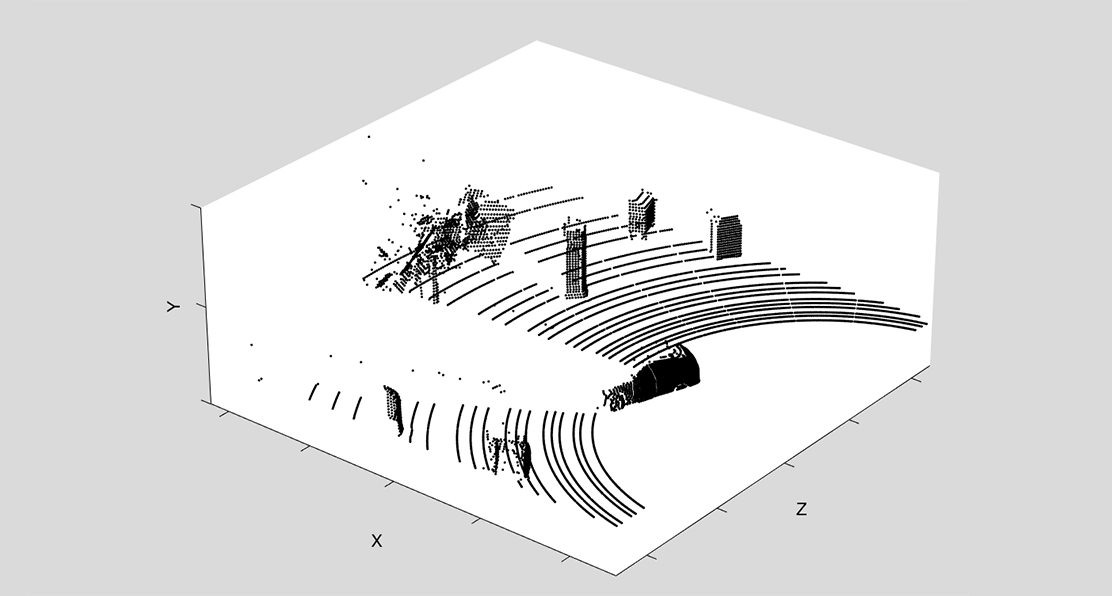
\includegraphics[width=0.8\textwidth]{./images/GC1.png}
%   \caption{An Overview of Data Set from Point Cloud of a single Scene}
%   \label{fig:data_overview}
% \end{center}
% \end{figure*}

%\usepackage{graphics} is needed for \includegraphics


% \begin{figure}%
% 	\centering
% 	\subfloat[point cloud readings simulated for a LiDAR sensor]{{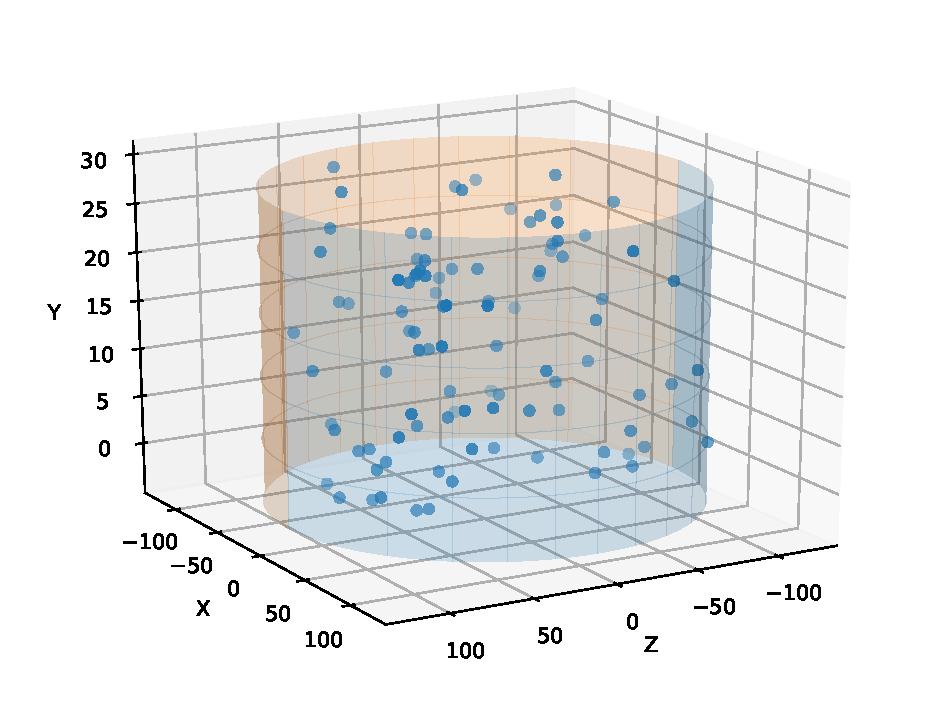
\includegraphics[width=7cm]{images/data_overview.pdf} }}%
% 	\qquad
% 	\subfloat[a scene with different numbers of objects]{{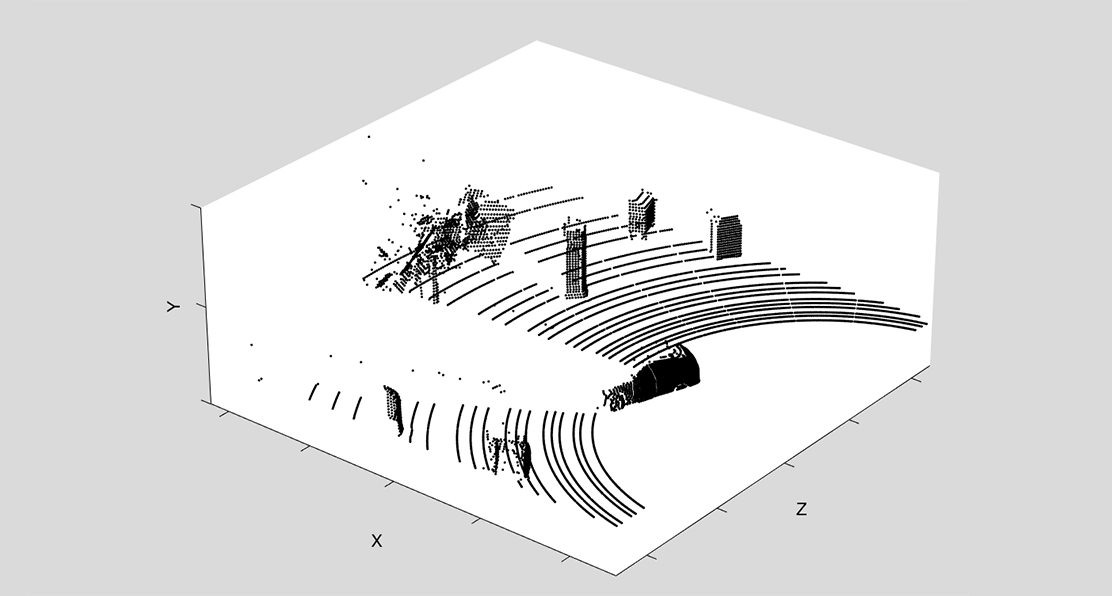
\includegraphics[width=5cm]{images/GC1.png} }}%
% 	\caption{An Overview of Data Set from Point Cloud of a single Scene}%
% 	\label{fig:data_overview}%
% \end{figure}


%KIA 
%Briefly describe the data set and cite the main grand challange paper. 

%We just need to describe what the data is about. 

% We need to mention other data sets like The KITTI Dataset \cite{Geiger2013IJRR}


% KITTI Dataset \cite{Geiger2013IJRR}

\section{Architecture}\label{sec:Architecture}




% Describe the data processing pipeline here. 


% 1. Get the raw data and remove the ground (LiDAR data clean up)
% 2. Segment data and sent it to classifier 
% 3. Classification with Neural Network. 


Figure \ref{fig:dataPipeline} depicts  

\begin{figure*}[h!]
 \begin{center}
   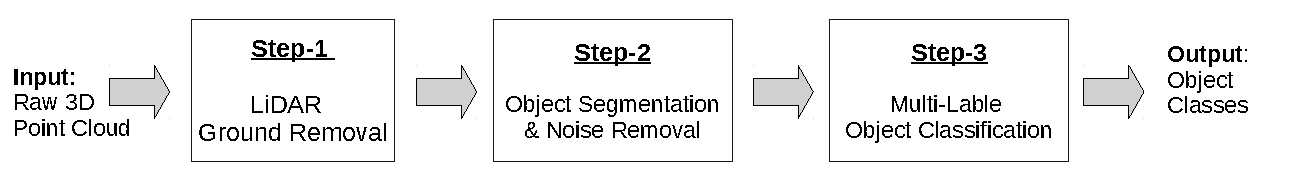
\includegraphics[width=0.9\textwidth]{./images/DataProcessingPipleline.pdf}
   \caption{An Overview of our Data Processing Architecture}
   \label{fig:dataPipeline}
 \end{center}
\end{figure*}





Describe \ldots. 

Different forms of data processing architectures that we have implemented and tested . 

\begin{enumerate}
  \item Different methods for removing noise from raw data (data preprocessing). 
  \item Projecting 3D data into 2D data using 3 different projection methods 
  \item CNN  (with and without maxpool) + fully-connected + dropout + fully-connected+softmax
  \item CNN with different number of hidden layers. 

\end{enumerate}



% KIA
% We need another image to describe the CNN architecture. 
% Add two images about it. 





\section{Evaluation}\label{sec:Evaluation}

\TODO{Describe the evaluation set up briefly.}



\TODO{- 3 Graph that compares the prcision/recall (F1) and time perofrmance of our multiple approaches. 
}


\TODO{Our appriaches are: 
1. Graphs for 2D CNN with simple linear projection on one of the axis.
2. 2D CNN with improved transformation from 3D to 2D CNN
3. 2D CNN - with - separation and projection and then segmentation with DBSCAN 
4. 3D CNN
5. Different No. of Layers up to 3 and 2 different size of filter. 
 }


- We should run it on a standard machine (better on EC2 because it is better reproducable) and show the processong time performance. 


- We present on our plots, Precision/Recall and Processing time. 





\section{Conclusion and Future Work}\label{sec:conclusion}













\bibliographystyle{ACM-Reference-Format}
\bibliography{refrences}




\end{document}
